%!TEX root =  proposal.tex

\section{Computational biology applications}


\subsection{Taxonomic classification of metagenomic data}

\textbf{Problem definition.}
The microbes that live in an environment can be identified by their combined genomic material, also called the metagenome.
The study of metagenomes provides an opportunity to closely examine complex biological interactions, such as phage-host and metabolic dynamics~\cite{national2007new}.
Metagenomic datasets contain sequencing reads from multiple species that are present in the biological environment.
%
Taxonomic classification~\cite{wood2014kraken} helps to identify the microbial taxon or taxa present in large-scale  metagenomic datasets coming from complex biological and environmental samples. Assigning taxonomic labels to sequencing reads is an important part of many computational genomics pipelines for metagenomics projects.

\noindent
\textbf{Importance.}
Metagenomic sequencing produces genomic data from a set of species instead of a pure species isolate, one of the primary challenges in the field is the development of computational methods for identifying all of the species contained in these samples.
%
Taxonomic classification of reads is a critical first computational step in any metagenomic analysis pipeline.
For example, read classification is critical for \emph{de novo} metagenomics assembly, which attempts to reconstruct the DNA sequence of each organism present in the metagenomic sample without using a reference database before performing the actual assembly step~\cite{venter2004environmental,brady2009phymm,brady2011phymmbl,rosen2008metagenome,segata2012metagenomic}.

\noindent
\textbf{Challenges.}
The task of read classification is far from straightforward.
A metagenomic sample can contain thousands of genomes with varying level of similarity and often occurring at vastly different abundances. Furthermore, due to high-throughput sequencing metagenomic datasets contains millions of sequencing reads making traditional, string-matching-based tools like BLAST infeasible to perform classification. Metagenomic datasets today easily range from hundreds of GBs to TBs~\cite{hofmeyr2020terabase}. For example, WA dataset contains a collection of marine microbial communities from the Western Arctic Ocean and consists of 822 GB of 2.5 billion reads in 12 samples~\cite{hofmeyr2020terabase}.
%
Although BLAST~\cite{altschul1990basic} is one of the most sensitive metagenomics alignment methods, it is computationally intensive, making it infeasible to run on the millions of reads typically generated by metagenomic sequencing studies.

\noindent
\textbf{State of the art.}
A large number of recently developed taxonomic classification tools~\cite{ames2013scalable, kim2016centrifuge, menzel2016fast, wood2014kraken, wood2019improved, dilthey2019strain,liu2018novel} use a supervised approach to assign taxonomic labels to reads.
These tools build a database of known previously sequenced microbial genetic sequences and their taxonomic labels from the NCBI database.
The database is typically an index (usually a compact hash table) that maps smaller subsequences (\kmers) to the list of taxa corresponding to the genomes in which the subsequences occur.
During the classification phase, the input reads are decomposed into \kmers and queried in the index to determine the most appropriate taxon using the lowest-common ancestor (LCA) of the genomes in the taxonomic tree.

\noindent
\textbf{Gaps and requirements.}
The sheer size of sequenced microbial genetic sequences presents a considerable computational challenge.
Building the database of known genomes is often quite memory intensive.
The most popular reference database are RefSeq complete genomes (RefSeq CG) for microbial species as well as the BLAST nt and nr databases for high-quality nucleotide and protein sequences, respectively, with $\approx50$ and $\approx200$ million sequences.
Kraken's~\cite{wood2014kraken} memory requirements can easily exceed 100GB~\cite{simon2019benchmarking}, especially when the reference data includes large eukaryotic genomes~\cite{meiser2017sequencing, knutson2017porcine}.
%
The universe of microbial sequences is large and diverse. The vast search space often results in false positives as sequences can be matched against multiple taxa. Also, a large number of undiscovered microbial species can result in false negatives as these species are not present in the database.

Existing taxonomic classification tools are memory intensive to build the database of known genomes and often require more memory than available on single-node machines. Furthermore, classification operation is computationally intensive and makes it infeasible to scale to terabyte-scale metagenomic datasets.
Second, this challenge is compounded by the exponential growth in recent years of the number of sequenced microbial genomes, meaning that the number of comparisons that need to be performed for new sequencing reads is huge and ever increasing.
%
Finally, existing reference database indexes give up updatability to save space. However, the ability to add new assembled genomes to an existing database is a critical feature to avoid rebuilding the databases.


\begin{rproblem}[\textbf{Metagenomic classification at terabyte scale}]
Build a software tool to perform reference-based taxonomic classification of metagenomic reads for terabyte-scale metagenomic datasets. The software tool will support adding newly sequenced microbial genetic sequences to the database and updating the labels of existing ones without rebuilding the whole database.
\label{rprob:taxo-meta}
\end{rproblem}

% \mfc{there is no discussion of what we are actually going to do.  what hardware?  what tests?  how will we know that we succeeded?  How much of an improvement do we need in order to succeed?  What it will it mean to our target application community if we succeed?}


\subsection{Large-scale raw sequence search}

\textbf{Problem statement.} Raw sequence search involves identifying all sequencing samples in a database of raw sequencing data such as SRA~\cite{kodama2012sequence,KatzSLKBO22} that contain a given query sequence. A query is an arbitrary sequence, such as a transcript. Raw sequencing datasets contain a ton of biological diversity information that can be used to answer biological questions that single sequencing sample do not have the power to address.

\noindent
\textbf{Importance.}
The Sequence Read Archive (SRA)~\cite{kodama2012sequence}, the world’s largest database of sequences, hosts approximately 10 petabytes (1016 bp) of sequence data and is growing at the alarming rate of 10 TB per day.
%
The vast majority of publicly available sequencing data (e.g., the data deposited in the Sequence Read Archive, or European Nucleotide Archive (ENA)~\cite{CumminsAABDEGHH22}) exist in the form of raw, unassembled sequencing reads. The raw sequencing data contains a lot of biological diversity information which is lost during the assembly process. Furthermore, only a small fraction of all the raw sequencing data is assembled, making the raw sequencing data even more important to answer complex biological-diversity related questions.
%
Enabling scientists to analyze existing sequence data will provide insight into ecology, medicine, and industrial applications~\cite{LeviRAE18}.
%
The genomics community established this database to enable sharing of the data, but the computational barrier to searching this data leaves the it separated from the people most qualified to analyze it.

\noindent
\textbf{Challenges.}
There have been multiple tools such as BLAST~\cite{altschul1990basic} and its variants that are designed to perform sequence level searches over publicly available databases of assembled genomes and known proteins. %Much subsequent work has focused on how to extend tools such as BLAST to be faster, more sensitive, or both~\cite{XXX}. \mfc{This previous sentence is a jolt. what does that have to do with raw sequence data?}
However, the strategies applied by such tools focus on the case where queries are issued over a database of reference sequences which is much smaller in size compared to the SRA\@.
Using BLAST (or other BLAST-based tools) to perform searches over SRA is computational not feasible.
%
There are a number of reasons that typical reference-database-based search techniques cannot easily be applied in the context of searching raw, unassembled sequences. One major reason is that most current techniques do not scale well as the amount of data grows to the size of the SRA (which today is $\approx4$ petabytes of sequence information). A second reason is that searching unassembled sequences means that relatively long queries (e.g., genes) are unlikely to be present in their entirety as an approximate substring of the input.
As such, these data have mostly been rendered impervious to sequence-level search, which substantially reduces the utility of such publicly available data.


\noindent
\textbf{State of the art.}
Recently, new computational schemes have been proposed that hold the potential to allow searching raw SRA while overcoming these challenges. Solomon and Kingsford~\cite{solomon2016fast} introduced the sequence Bloom tree (SBT) data structure and an associated algorithm that enables an efficient type of search over thousands of sequencing experiments. Specifically, they re-phrase the query in terms of k-mer set membership in a way that is robust to the fact that the target sequences have not been assembled. The resulting problem is coined as the experiment discovery problem, where the goal is to return all experiments that contain at least some user-defined $q$ fraction of the \kmers present in the query string.
%
Subsequently, Mantis~\cite{PandeyABFJP18Cell} was developed by PI Pandey and PI Bender that showed how solve the experiment discovery problem using an inverted-index approach by mapping \kmers to the list of experiments they appear in. Mantis uses the counting quotient filter~\cite{PandeyBJP17} as an exact map to map \kmers. Mantis's index is smaller in size, faster to index and query, and has no false positives compared to the SBT (and other SBT-based tools~\cite{SolomonK17,HarrisM20,BingmannBGI19}).
%
PI Pandey further continued this effort in collaboration with Prof.\ Patro (UMD) to compress the Mantis index in order to reduce memory requirements and scale Mantis~\cite{AlmodaresiPFJP19,AlmodaresiPFJP20} to storage devices.


\noindent
\textbf{Gaps and requirement.}
Existing raw sequence search indexes suffer from the scalability challenge. Indexing \kmers from the SRA samples is memory intensive and indexes often take hundreds of GBs. For example, the SBT index size for 2652 experiments consisting of short-read RNA sequencing runs of human blood, brain, and breast tissues is 97~GB\@. Scaling SBT-based indexes to 100K experiments in SRA is not feasible on single-node machines.
Furthermore, SBT-based indexes are approximate the search results include false positives which can quickly become problem even if 1\% results are false positives due to the shear size of the search space.

Mantis index is exact and has no false positives in the results. Recently, LSM-Mantis~\cite{almodaresi2022incrementally} showed how to efficiently scale the index to SSD storage devices using the~\cite{BentleyS80}. However, even LSM-Mantis could only index 40K experiments from the SRA\@. These indexes are reaching the limits of single-node RAM and storage hardware.

\begin{rproblem}[\textbf{Build a raw sequence search index over all of SRA}]
Build a \kmer index over all the raw experiments present in SRA and enable sequence-level searches in real-time. Furthermore, host the index publicly to make it available for researchers around the world.
% Researchers can quickly ask biological questions and get answers.
% For example: what if researchers wants to determine: if a new putative disease-related transcript appeared in other samples, if a new fusion event is common among samples with a given subtype, which samples contain a new unexpected bacterial contaminant.
\label{rprob:seq-search}
\end{rproblem}

\subsection{Pangenomics}

\textbf{Problem definition.}
Pangenomics~\cite{sherman2020pan} involves cataloging the DNA of multiple individuals in a species in the form of a sequence graph to preserve the variation across the individuals in a species. This pangenome is used as the reference genome for the species and forms the basis of thousands of studies seeking the genetic origins of diseases. In pangenomics, we need to efficiently index the variations (SNPs, indels, copy number, structural, etc.) and support variant queries. Furthermore, we need to perform sequence-to-graph alignment to determine new variants.


\noindent
\textbf{Importance.}
Much of the field of genomics revolves around the existence of reference genomes, which are roadmaps for a ‘typical’ individual of each species.  However, as the number and scope of sequencing experiments have grown dramatically, scientists have begun to realize the many limitations that a single reference genome imposes upon the community. To better capture the variation missed by using one reference, we can create and utilize a ‘pan-genome’, a collection of all the DNA sequences that occur in a species.
A primary goal of pangenomic variation analysis is to avoid biases that arise when treating a single genome as the reference when identifying or comparing variants across samples in a population.
The first pan-genomes were developed for small, easy-to-sequence bacteria, but, even in that context, pan-genomes provided novel scientific insights. The consideration of genetic diversity within bacterial species has contributed to our understanding of underlying differences in pathogenicity, virulence and drug resistance and can even help predict how pathogenic a new strain will be~\cite{sherman2020pan}.

\noindent
\textbf{Challenges.}
Cataloging the DNA from all individuals in a species is a daunting task.
Building a pangenome graph involves storing the genomic sequences of thousands individuals in the form of a sequence graph. Each path in the sequence graph follows the genome of an individual and has a unique coordinate system. A coordinate systems helps to identify the location of a variant in the genome of an individual. Due to the presence of insertions and deletions in genomes across individuals, each individual can have a unique coordinate system~\cite{pandey2021variantstore}.
During variant queries, we need to identify a variant with respect to an individual's coordinate system due to the absence of a reference genome.
A Pangenome consists of thousands of individuals and hence thousands of coordinate system in a single index. Indexing and querying the pangenome graph across thousands of coordinate system is computationally and memory intensive and requires scale up and scale out solutions~\cite{garrison2018variation,pandey2021variantstore}.

\noindent
\textbf{State of the art.}
Pangenomic studies are performed by storing the genomes of multiple individuals in a genome graph (also known as the sequence graph or variation graph). A genome graph is a directed, acyclic graph (DAG) $G = (N, E, P)$ that embeds a set of DNA sequences. It comprises a set of nodes $N$, a set of direct edges $E$, and a set of paths $P$. For DNA sequences, we use the alphabet \{A, C, G, T, N\}\@. Each $n_i \in N$ represents a sequence $seq(n_i)$. Edges in the graph connect nodes that are followed on a path. Nodes on a path are assigned positions based on the coordinate systems of sequences they represent.

% Efficiently indexing and storing a genome graph is a computationally and memory/space intensive process due to the presence of thousands of coordinate systems corresponding to the individuals.
Existing applications that index genome graphs~\cite{pandey2021variantstore,garrison2018variation} are designed to use compressed string indexes and off-the-shelf graph indexes. VG toolkit~\cite{garrison2018variation} is one of the most widely used tools to represent genomic variation data, and it also supports multiple coordinate systems. VG toolkit stores each sample path as a list of nodes in the graph and maintains a separate index corresponding to the coordinates of the reference and samples.
%
VariantStore~\cite{pandey2021variantstore}  encodes genomic variation in a directed, acyclic variation graph and build a position index (a mapping of node positions to node identifiers) on the graph to quickly access a node in the graph corresponding to a queried position. It builds an inverted index from variants to the nodes in the graph to achieve space-efficiency due to repeated variants and fast variant queries.

\noindent
\textbf{Gaps and requirement.}
Current pangenomic indexes do not scale to population-scale variation datasets such as 100,000 Genomes project~\cite{1002021100}. For example, VG toolkit stores each sample path as a list of nodes in the graph and maintains a separate index corresponding to the coordinates of the reference and samples. Storing a separate list of nodes for each sequence impedes the scalability of the representation for storing variation from thousands of samples. Moreover, variants are often shared among samples, so storing a list of nodes for each sample path introduces redundancy in the representation.
%
Existing pangenome indexes do not support adding new genomes to an existing index. In order to add a new genomic sample to the pangenomic index required rebuilding the complete index. For example, both VG toolkit and VariantStore are static indexes and do not support an efficient approach for adding new genomes to an existing index.

Finally, pangenomic indexes need to support fast variant queries and sequence-to-graph alignment. Achieving both these operations in a single index is a challenging task. Existing tools are optimized for one of these operations but not both. VG toolkit is designed for fast sequence-to-graph alignment and VariantStore for variant queries.


\begin{rproblem}[\textbf{Building a pangenomic index at population-scale }]
 Build a pangenomic index that can perform fast variation queries and sequence-to-graph alignment at population-scale datasets available today. We further want to support adding new genomic samples to an existing index without rebuilding the index.
\label{rprob:pangenomics}
\end{rproblem}

\subsection{Metagenome assembly}
\prashant{Revisit this subsection \ldots}

% \begin{figure}
% \begin{wrapfigure}{R}{0.7\textwidth}
%     \centering
%     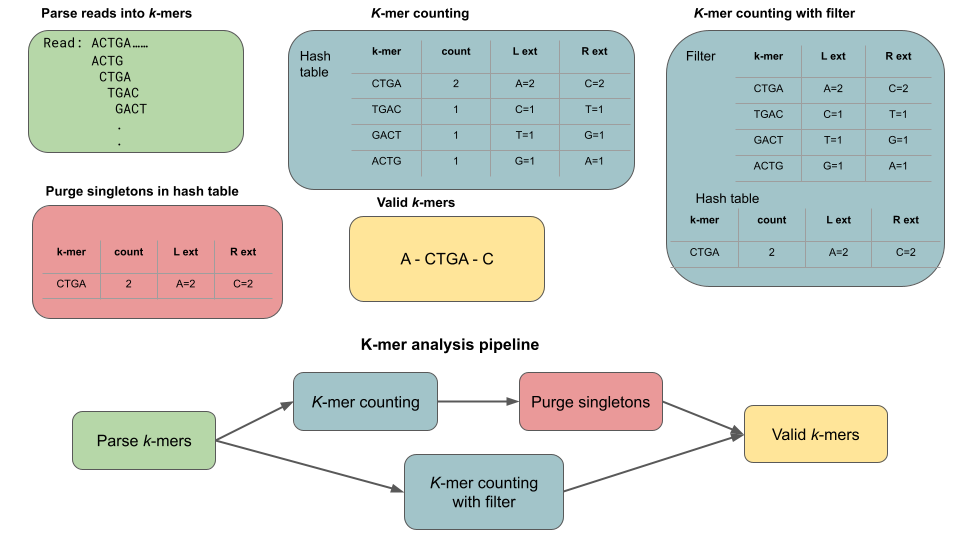
\includegraphics[width=0.9\linewidth]{images/mhm-pipeline.png}
%     \caption{The \textit{k}-mer analysis pipeline in MetaHipMer. A filter can help weed out singleton \kmers from being inserted into the hash table.}
%     \vspace{-0.5em}
%     \label{fig:mhm-kmer}
% \end{wrapfigure}
% \end{figure}

\textbf{Problem definition.}
Metagenome assembly involves reconstructing long contiguous sequences (\emph{contigs}) of genetic material from short input \emph{reads}~\cite{yang2021review}. These reads are strings of bases (the DNA alphabet A, C, G, T) of length 150 to 250 that are produced by gene sequencing machines.
For metagenomes, these reads are extracted from environmental samples (e.g., gut bacteria, or a soil sample) that contain the genes of potentially thousands of microbes, existing at varying abundances.
The reads are error-prone (typically about 0.24\% error per base) and sequencing is done multiple times to ensure every region of genetic material is covered with some error free sequences.

\noindent
\textbf{Importance.}
Metagenomic sequencing provides a culture-independent avenue to investigate the complex microbial communities by constructing metagenome-assembled genomes (MAGs). A MAG represents a microbial genome by a group of sequences from genome assembly with similar characteristics. It enables us to identify novel species and understand their potential functions in a dynamic ecosystem.

\begin{wraptable}{r}{4.5in}
\centering
%\resizebox{\columnwidth}{!}{%
    \begin{tabular}{c | c | c | c | c | c}
    \toprule
    \textbf{Dataset} & \multicolumn{5}{c}{\textbf{Percentage singleton \kmers}} \\
    \midrule
    & $K=21$ & $k=33$ & $k=55$ & $k=77$ & $k=99$ \\
    \midrule
    WA &  66 & 73 & 76 & 78 & 78  \\
    Rhizo &  67 & 75 & 80 & 83 & 85  \\
    Tymeflies & 63 & 62 & 67 & 69 & 71 \\
    \bottomrule
    \end{tabular}
 %   }
    \caption{Distribution of singleton \kmers in metagenomic data for values of $k$.}
    \label{tab:kmer-dist}
\end{wraptable}

\noindent
\textbf{Challenges.}
Metagenome assembly is challenging due to sequencing error, repetitive content, and library and sequencing bias. In addition, a metagenome sample can contain many thousands of different genomes with varying degrees of similarity, sometimes sharing genetic material, and occurring at vastly different abundances.
%
Furthermore, high-throughput sequencing technology is producing large-amount of metagenomic datasets ranging in TB and PB scales~\cite{hofmeyr2020terabase}. Metagenomic assembly is a complex process consisting of multiple phases and scaling all these phases to terabyte scale comes with myriad of challenges.

\noindent
\textbf{State of the art.}
MetaHipMer~\cite{GeorganasEHG18,hofmeyr2020terabase} is the first exascale metagenome assembler.
In the approach used by MetaHipMer, the reads are first divided into overlapping substrings of fixed length \emph{k}, called \emph{\kmers}, which are then used to form a de Bruijn graph~\cite{CompeauPeTe11}.
\Kmer counting is the very first step. During \kmer counting, forward and backward extensions of the \kmer and the counts of those extensions are also maintained in the hash table along with the \kmer. Information regarding the extensions and their counts is critical to identifying correct paths in the de Bruijn graph and requires 28 to 52 bytes (depending on $k$) to store each \kmer.
MetaHipmer uses GPUs to speed up \kmer analysis phase.
In a de Bruijn graph, the vertices are \kmers and edges connect any two \kmers that have an overlap of $k-1$ bases. These vertices are stored in a hash table that is distributed across all the compute nodes in a supercomputer like Perlmutter~\cite{perlmutter} and Summit~\cite{summit}.
Traversal of the de Bruijn graph enables the construction of the contigs (longer sequences).  This approach is more efficient than an all-to-all alignment of the reads, which would be prohibitive for the size of typical metagenome datasets (up to billions of reads).

\noindent
\textbf{Gap and requirements.}
\Kmer counting and analysis is the very first and the most memory intensive step in the metagenome assembly. The \kmers that occur only once (singletons) are treated as sequencing errors and dropped. In a typical set of metagenome reads, 70--80\% of unique \kmers are singletons, but they still need to be stored and counted in the distributed hash table~\Cref{tab:kmer-dist}.
In the default MetaHipMer implementation, storing the unique \kmers is the most memory intensive part of the computation and can be roughly an order of magnitude larger than the input data.  The space required to store the \kmers can be much larger than the size of the original raw dataset (up to $10\times$ larger) as \kmers contain a lot of redundant information due to their overlaps.
Weeding out singleton \kmers before inserting them in the hash table to count is critical in any \kmer analysis phase to reduce the memory usage of the counting phase. These singleton \kmers can also be pruned from the hash table after the counting phase. However, that results in the high peak memory usage and much slower running time. MetaHipMer uses filers to weed out singleton \kmers.

The size of the filter and hash table is dependent on the number of unique \kmers. Given that the distribution of \kmers is highly skewed and not known in advance, it is challenging to size the filter and the hash table in order to efficiently utilize the limited memory. Filter and hash tables that can be efficiently resized at run time will enable efficient memory utilization.


\begin{rproblem}[\textbf{Scale MetaHipMer to petabyte-scale metagenomic datasets on supercomputers}]
Accelerate \kmer analysis phase in MetaHipMer using GPUs and reduce the peak RAM usage to support assembly of petabyte-scale metagenomic datasets from complex biological environments.
\label{rprob:metahipmer}
\end{rproblem}
